\documentclass[12pt,a4paper]{article}
\usepackage{natbib}         % Pour la bibliographie
\usepackage{url}            % Citation des adresses web
\usepackage[T1]{fontenc}    % Encodage des accents
\usepackage[utf8]{inputenc} % Encodage des accents
\usepackage[frenchb]{babel} % Pour la traduction française
\usepackage{numprint}       % Affichage correcte des chiffres
\usepackage{titlesec}
\usepackage{graphicx}
\title{Projet de Programmation Numérique : Extension de la Résolution de Noms pour le HPC\\}
\author{YEHOSSOU Kakpo, KONÉ Sirata, MLARAHA Hassan}
%\date{}

\begin{document}

\maketitle

\newpage
\tableofcontents
\listoffigures
\newpage

\newpage
\section*{Introduction}
\addcontentsline{toc}{section}{Introduction}

\quad Dans le cadre du projet de programmation numérique, il nous a été demandé de réaliser un proxy DNS avec des fonctionnalités étendues, permettant de couvrir les besoins en résolution de noms pour des machines parallèles dédiées au calcul haute performance, sur une architecture distribuée.

\quad Nous présenterons dans une première partie le projet de manière générale, à savoir le contexte et les objectifs à atteindre. Ensuite, nous expliquerons plus en détail la conception et les implémentations effectuées. Puis, nous expliquerons notre organisation et la répartitions des tâches. Enfin, nous aborderons un point de vue critique sur l’ensemble de la solution élaborée, ainsi que les améliorations envisageables.

\newpage
\section{Présentation générale}
Ce projet se présente sur plusieurs axes principaux à savoir :
\subsection{Contexte du projet}

\quad Dans le domaine du calcul haute performance, la communication entre machines (ou des processus) est l’une des préoccupations les plus importantes en terme d’optimisation. En effet, les entités parallèles doivent être en mesure de pouvoir mener à bien les opérations complexes qui leurs sont assignées, et ceci quelque soit la configuration de l’architecture (partagée ou distribuée) afin de résoudre le problème posé.

\quad Pour s’échanger des données, les processus parallèles (jusqu'à plusieurs millions) doivent au préalable être capable de s’identifier et de se reconnaître les uns par rapport aux autres, afin de s'interconnecter, et ce de la manière la plus efficace possible. C’est en ce sens qu’un mécanisme de résolution de noms performant est essentiel pour l’identification de ces entités. Dans le cas des réseaux de machines distribuées, des solutions existent pour accomplir cette nécessité. Dans les sections suivantes, nous présentons deux de ces solutions : le PMIx et le DNS qui agissent souvent de manière complémentaire lors du lancement des applications parallèles.

\subsubsection{Le Standard PMIx}

\quad L’interface PMIx (\textit{Process Management for Exascale Environments}) est une API (\textit{Application Programming Interface}) et plus récemment un standard qui fournit un accès portable et bien défini aux services communément utilisés par les systèmes de calcul distribué. Plus précisément, la PMIx implémente un stockage clef-valeur distribué permettant l'échange des informations de connection lors du lancement des programmes MPI. De plus, ce stockage est généralement géré par le batch manager, et donc présent avant que le programme ne soit lancé, agissant alors comme tiers de connectivité.

\quad Cette interface a été développée et distribuée dans le cadre du projet MPICH (implémentation portable et \textit{open-source} de la bibliothèque de calcul parallèle MPI). À l’origine, elle était utilisée comme moyen de communication (filaire) entre processus, et également comme un outil de déploiement de processus. L’API  a connue plusieurs versions respectivement appelée PMI1, 2 et plus récemment X pour Exascale. Cette dernière fait l'objet d'un processus de standardisation cf. \url{pmix.org}.

\quad Plus précisément, PMIx intervient lors du lancement des programmes MPI (et plus généralment distribués) pour:
\begin{itemize}
    \item Donner le nombre de processus lancés (rank et size);
    \item Permettre l'échange des informations de connexion (point d'intérêt dans notre étude);
    \item S'interfacer avec le batch manager pour lancer des processus dynamique.
\end{itemize}

L'objet de notre étude sera d'étudier la convergence de DNS avec PMIx afin de déterminer s'il existe des symétries entre ces deux services, et donc un moyen de les coupler.

\subsubsection{Le protocole DNS}

\quad Le protocole DNS (\textit{Domain Name Service}) est un mécanisme qui permet d’obtenir l’adresse IP d’une machine à partir d’un nom de domaine (sous la forme d’une URL), ou le nom de domaine d’une machine à partir d’une adresse IP. Dans le second cas, on parle de résolution inverse. La conversion entre nom de domaine et adresse IP est possible grâce à la mise en place d’un espace de noms hiérarchisé. Ce dernier est organisé sous la forme d'un arbre à plusieurs niveaux, calqué sur la structure des organismes gouvernementaux et non-gouvernementaux. Le caractère "." est utilisé pour marquer la frontière entre deux niveaux hiérarchiques.

\quad La création de ce protocole à une importance dans l’existence d’Internet tel que nous le connaissons à l’heure actuelle. En effet, en 1983, les protocoles TCP et IP ont été adoptés pour identifier les machines hôtes du réseau ARPANET (\textit{Advanced Research Projects Agency Network}). La résolution de noms était réalisée par l’intermédiaire d’une table de correspondance entre noms d’hôtes et adresses IP. Cette table était enregistrée dans le fichier \textit{hosts.txt} (ancêtre de \textttt{/etc/hosts}, ce dernier étant maintenu par le NIC (\textit{Network Information Center}). La transmission du fichier était effectuée via le protocole FTP à tous les hôtes du réseau. C’était alors les débuts d’Internet.

\quad Avec l’augmentation exponentielle du nombre de machines hôtes, la mise à jour du fichier \textit{hosts.txt} devenait complexe (encombrement de la bande passante du NIC). De plus, la croissance d’Internet étant inévitable, les divers organismes impliqués ont exprimé leur besoin d’autonomie dans la gestion de leurs communications à travers ce réseau. Dans ce contexte, Paul Mockapetris et John Postel développent entre 1983 et 1984 une solution qui utilise des structures de base de données distribuée : les \textit{Domain Name Systems} (RFCs 882 et 883, aujourd’hui obsolètes). Cette première approche aboutit en novembre 1987 à la spécification du protocole DNS (RFCs 1034 et 1035).

\qaud Ainsi, le DNS a été créé avant tout pour rendre le plus agréable possible la communication entre les machines du réseau Internet.

\subsection{Objectifs du projet}

\quad Comme énoncé dans le préambule de cette partie, la principale problématique consiste à trouver un moyen efficace et scalable d’interconnecter des processus entre eux, par intermédiaire d’un système de résolution de noms. En d'autres termes nous souhaitons étudier une convergence possible entre la Process Management Interface (PMI) et le protocole DNS. En effet ils ont des rôles comparables, permettre à des machines de se retrouver, l'un est temporaire à un job donné l'autre est souvent un service allant du calculateur lui même (cas d'un réseau isolé) à l'Internet mondial.

\quad L’interface PMIx, qui propose des diverses solutions portants sur les systèmes de calcul distribué, fournit déjà à sa manière un système de résolution de noms. Cependant, le protocole DNS, qui constitue actuellement la norme du réseau Internet pour la résolution de noms de domaine et d’adresses IP, a fait ses preuves en termes d’efficacité pour l’identification de machines. Ainsi, la connectivité TCP (IPV4,6) est déjà portée par DNS, ce qu'il manque alors est une gestion de clefs étendues pour l'échange d'informations non IP (par exemple pour Infiniband). De plus, le DNS a un scope machine (le plus souvent) et donc il nous faut considérer un stockage temporaire attaché à un job donné, d'où l'idée de \emph{proxy DNS} qui sera développée par la suite. Enfin, particulièrement si le programme est amené à faire aussi du TCP, la PMI peut amener à des résolution DNS par la suite, si on stocke le nom d'hôte dans le clef-valeur (et non l'IP) car faire cette résolution à l'avance est non trivial (déterminer la route vers l'hôte donnée).

\quad Dans ce contexte, l’objectif principal de notre projet consiste à réaliser un proxy DNS dans l’optique de renforcer et d’étendre les capacités de résolution de noms de l’interface PMIx. L’optimisation de notre solution ainsi que la mise en place d’un système de cache est également envisageable.
Dans les grandes lignes, nous devons :
\begin{itemize}
    \item Étudier le protocole DNS et ses implémentations (recherches et documentation) ;
    \item Créer un client, un serveur et un proxy DNS en utilisant les appels de la \textit{libc} (\textit{getaddrinfo...}) ;
    \item Ajouter des fonctionnalités supplémentaires à notre solution DNS (utilisation du champ \textit{TXT}) ;
    \item Effectuer des tests de validation et de performance pour évaluer notre solution.
\end{itemize}

Les principales motivations pour la réalisation de ce projet sont les suivantes :

\begin{itemize}
    \item Mettre en évidence le rapprochement entre la résolution de noms et le mécanisme de clé/valeur de la PMIx ;
    \item Implémenter un proxy DNS fournissant également les capacité de la PMI;
    \item Unifier DNS avec la PMI tout en rendant le tout scalable.
\end{itemize}

\newpage
\section{Implémentations}

\subsection{Fonctionnement du proxy DNS}

\quad Un serveur proxy est un intermédiaire entre le client et l'internet. La requête du client passe par lui et vis versa. Si nous nous plaçons dans le cas où nous avons un client d'un côté, un serveur de l'autre. Ainsi, nous proposons de complément le DNS en nous insérant au milieux entre le client (le programme MPI) et le serveur (celui de la machine). De cette manière nous créons un espace de nom temporaire (attaché au job) dans lequel nous pouvons fournir les fonctionnalités de PMI et de DNS via un service auto-porté. Pour commencer un ensemble de processus donnés et à terme les processus MPI eux même en peer-to-peer.\\

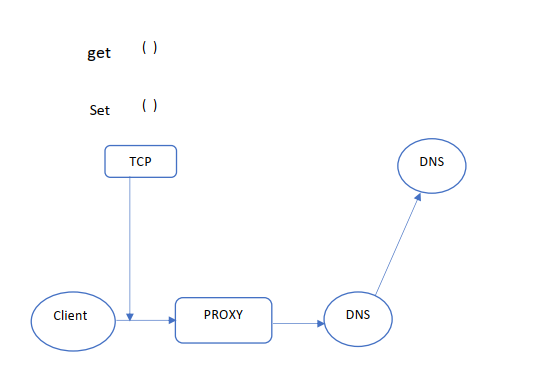
\includegraphics[scale = 0.5]{figures/Capture.PNG}
\captionof{Figure 1}{ : Figure explicative du rôle d'un bref rôle du proxy}
\\
\subsubsection{Les structures de données et routines associées}

Le proxy DNS est finalement un programme simple, dans un premier temps nous avons adopté un protocole ad-hoc en TCP pour supporter nos requêtes. Le client se connecte au serveur qui maintient une table de hachage des différentes clefs. De plus, si une clef est inconnue, la résolution DNS est tentée (via getaddrinfo) afin de retourner une résolution DNS, cette même résolution et stockée dans la table pour optimiser une réponse future, agissant alors comme un cache DNS.

\subsubsection{La communication client/serveur}

La communication Client Serveur est privilégier ici dans notre cas pour résoudre le problème de surcharge en fin de rendre plus performant les requête étant donnée que si nous avons ses millier de machines connecter nous pourrons être confronté à un grand problème de scalabilité. En particulier l'objectif final de ces travaux est de fournir une PMI couplée à un DNS performant. De ce fait, pour répondre à un grand nombre de clients il faut potentiellement un grand nombre de serveurs, encourageant une architecture distribuée.\\
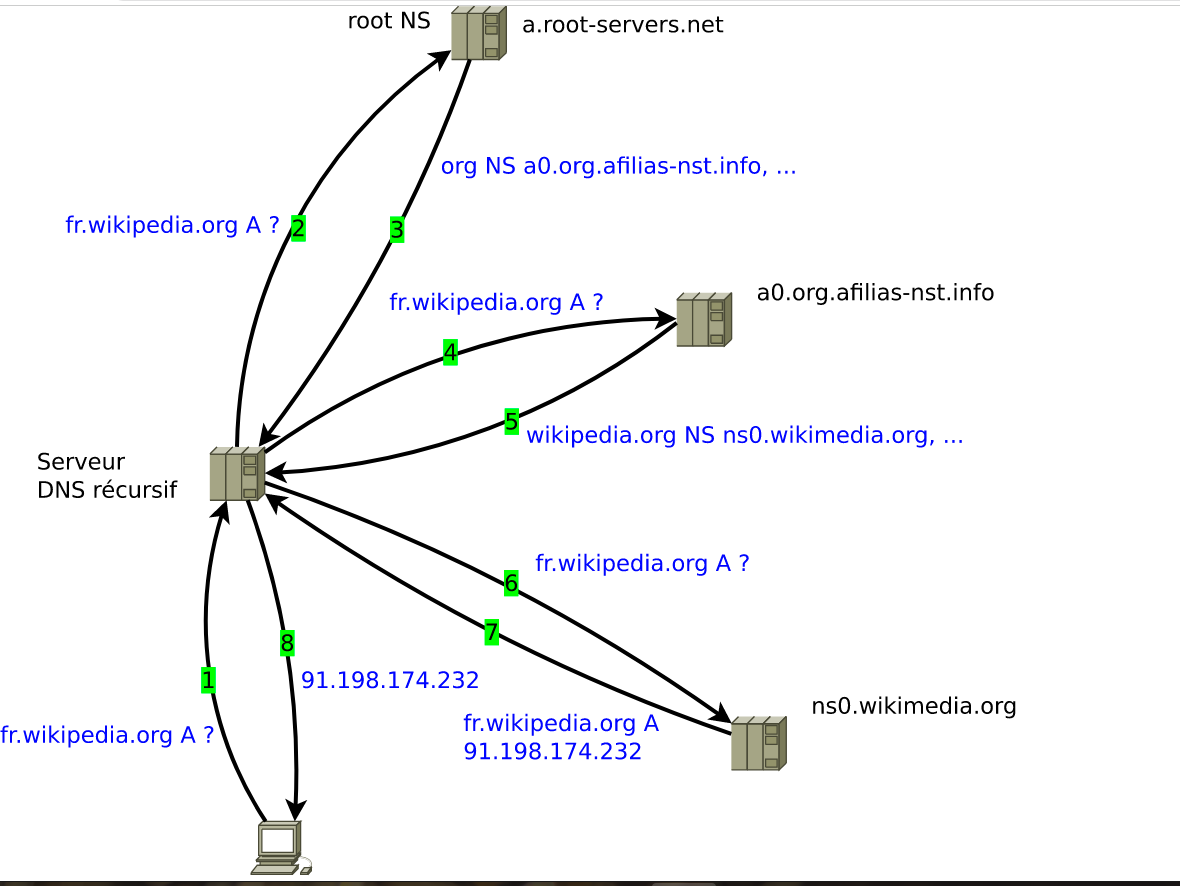
\includegraphics[scale = 0.4]{figures/wiki.png}
\captionof{figure 2}{ : Tirer de wikipedia}
%\label{Figure1}\\
Cette figure explique comment un client questionne un serveur DNS et de manière récursive comment la réponse est trouver et lui est retransmise à la $8^ème$ étape sur la figure1.\\
\subsection{Principe de la table de hachage}
\quad La table de hachage est une forme de stockage des données utilisant un algorithme qui est tableau. Comme son nom l'indique, cette table repose sur une fonction de hachage afin de calculer par une opération mathématique une cellule (de manière unique pour une clef donnée) de plus, cette cellule contient autres tables afin de parer aux collisions(car la table principale est de taille finie). De cette manière la table a une complexité de recherche inversement proportionnelle à sa taille. En effet, la recherche elle en a une complexité au pire des cas une complexité en $O(p)$ avec $p$ le nombre de table inférieur à nombre d'élément/10, ici la table de hachage permet une complexité moyenne en $O(p)$. Ainsi, cette structure de donnée est tout à fait adaptée à l'implémentation d'un stockage clef-valeur.

%\subsubsection{Choix d'implémentation}

%\quad Nous avons estimer qu'en utilisant juste un tableau et en considérant le pire des cas, en faisant une recherche en parcourant tout le tableau nous pouvons avoir une très bonne performance si nous avons une taille de tableau relativement très petit. Dans le cas où nous aurons un tableau assez grand, là un problème de performance se pose.

%\quad Avec la table de hachage, en connaissant l'indice, nous accédons directement à l'élément. Dans le cas où les indice se répète, nous aurons à parcourir l'élément suivant jusqu'à obtenir l'élément recherché sinon nous reprenons depuis le début du tableau.

%\quad Peut être qu'il serai mieux après d'utiliser un tableau, mais plusieurs processus pour le contrôler en divisant le tableau en petite table inférieur ou égale à 7 éléments.

\subsection{Interface Clef-Valeur}
C'est une forme d'implémentation qui est basé sur des tableau, facilitant ainsi l'accès à toute la donnée d'un emplacement quelconque de ces donnée à partir d'une information qui peut être clé ou valeur. Elle facilite aussi le stockage des données sous la forme de clé et valeur. Ici elle prend en compte trois principale opérations.

\subsubsection{Opération \textit{Get}}

\quad Initialement si un programme MPI se connecte, il fait un "get size" et un "get rank". Donc pour un rang, il doit faire un "put" de son identifiant et les autres qui veulent se connecter à lui feront un "get", et c'est PMI qui fait l'échange. Ici, la fonction get est une fonction qui prend une valeur se présentant sous forme de caractère qui pourrait être un clé selon notre implémentation. Le "get" permet donc d'obtenir une valeur qui est retourner par le serveur grâce à un système de fichier ou de cache. La valeur peut être l'IP associée à la clé qui pourrait être à son tour le nom ou un identifiant. Dans le cas ou cette valeur n'existe pas sur le système de fichier ou sur le cache, une requête DNS est lancer pour résoudre le nom.

\subsubsection{Opération \textit{Set}}

\quad Pour stocker une clé (nom et identifiant) et une valeur nous utilisons la fonction "set". Donc un client en se connectant pourra faire un "set" pour ajouter à la table existante une nouvelle machine (nom et identifiant ou IP).

\subsubsection{Opération \textit{Delete}}

Enfin, la fonction delete permet de retirer une clef du stockage clef-valeur.

%\subsection{Autres Opérations}

%\subsubsection{Résolution inverse}

%\quad La résolution inverse une une autre opération qui prend une valeur en entrée et retourne la clé. c'est à dire retourne le nom associé à la valeur. Lorsqu'elle n'existe pas, une requête DNS inverse est réalisée par le serveur pour retourner une réponse DNS.\\
%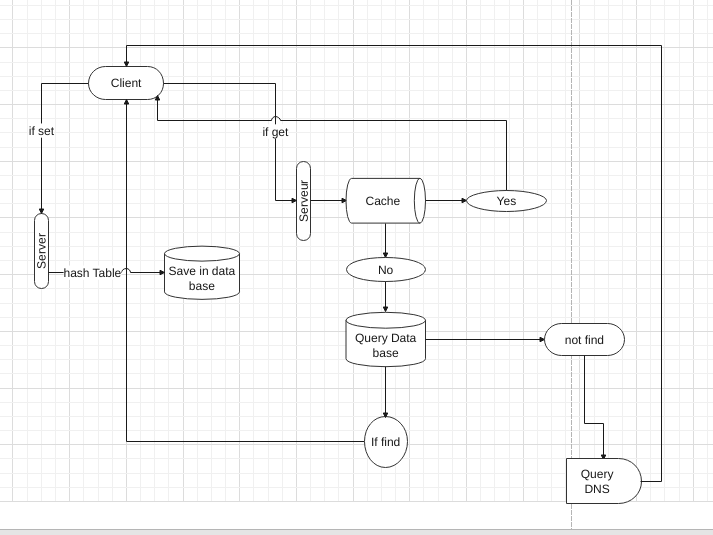
\includegraphics[scale = 0.5]{figures/hashtable_img.png}
%\captionof{Figure 3}{ : Figure expliquant le fonctionnement de la table de hachage suite à de différentes requêtes}\\
\subsection{Système de \textit{log}}

\quad Notre système de \textit{log} fonctionne en deux mode : écriture et lecture. Tout d'abord, on déclare deux variables : "char ip" et "char port", ainsi qu'un entier. On demande avec la fonction "fprintf" d'afficher l'adresse IP du client. On utilise la fonction "gets", qui nous permettra d elire le tableau directement. On fait de même pour le port et le numéro de PC.

\subsubsection{Traitement du fichier}

\quad Premièrement, nous avons fait une fonction qui écrit dans un fichier fonctionnelle. Ici, le plus important
pour la déclaration du fichier, nous faisons appel a "FILE *f" et nous l'affectons à la valeur "NULL". On ouvre notre fichier en mode écriture en faisant appel a la fonction "fopen". Cette dernière va le mode. Voici le différents modes :
\begin{itemize}
    \item r {lecture seule, mais le fichier doit exister}
    \item w {écriture seule}
    \item a {ajout fin fichier}
\end{itemize}

\quad Il y en a beaucoup comme w+ ou r+ ou a+, mais nous, on utilise le mode r ici pour éviter la fuite de mémoire vis-à-vis de la fonction "gets" qui est un peu dangereuse. Pour créer et écrire dans un fichier, nous avons utiliser le mode "w". Enfin, nous pouvons récupérer les informations existantes dans notre fichier. Pour cela nous utilisons le mode "r" et la fonction "scanf".

\newpage
\section{Choix d'implémentation et Mesure de Performance}
\subsection{système de cache}
\subsubsection{table de hachage}
\quad Le choix d'une fonction de hachage simple mais efficace réside du faite que nous cherchons à construire un système de clé valeur efficace or nous estimons avoir un très grand nombre de données donc il est important de trouver un algorithme de hachage dont les collisions pourraient considérablement réduite en fonction de l'augmentation de la taille des données. Ce qui répond parfaitement au comportement de notre fonction de hachage qu'on pourra observer sur la figure suivante.\\\\
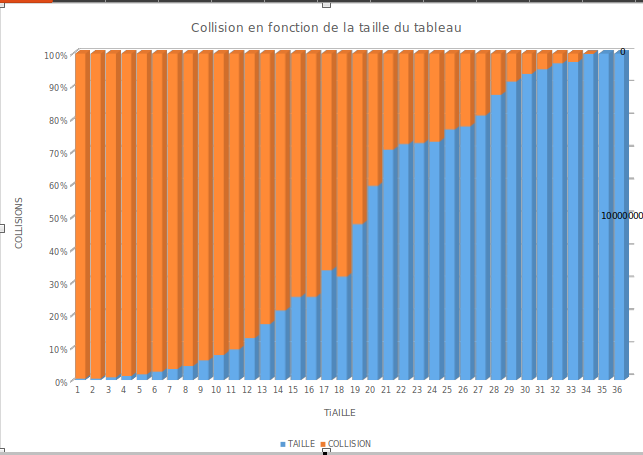
\includegraphics[scale = 0.5]{figures/collision.png}\\
\captionof{Figure 3 }{ :  Explicative de l'évolution des collisions en fonction de la taille du tableau}
\subsubsection{Sérialisation des données en échange}
\qaud L'échange de données sans perte de bout en bout étant très important en réseau, nous avons pensés à assurer cette fonctionnalité de transmission sans perte de données.
\subsubsection{Test de validation}
\qaud Assurer des entrés et sortir de nos différentes fonctions, il est donc important de les faire validées.
\subsection{Parallélisation et Performance}
\subsubsection{Table de hachage}
\quad En séquentiel, Le programme n'assure pas un accès ordonné des différentes ressources, nous avons constaté dans un premier temps qu'ils peut y avoir le stockage de la même donnée à de différents endroit au cour de la même opération d'insertion. Alors donc une suppression non complète des donnée de la table.
\qaud Pour eviter les effet de bort, des resultats nom attendu, il est important de protéger l'accès de données de notre tableau.
\qaud Cela nous amène à perdre en performance mais que Ce soit la version séquentielle ou parallèle nous avons une meilleur performance qu'une requête DNS:\\\\
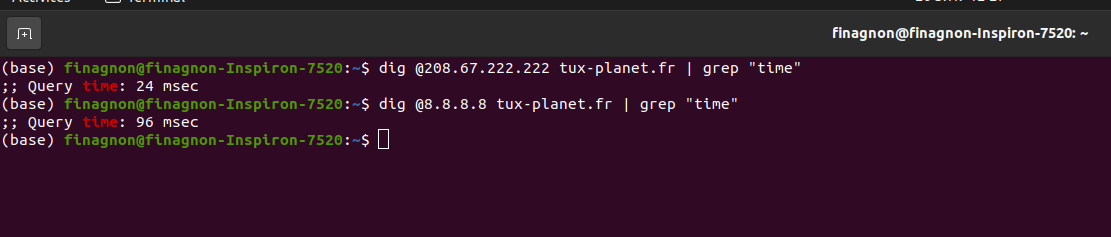
\includegraphics[scale = 0.5]{figures/dig.png}

\captionof{Figure 4}{ : Montrant le temps d'une requête DNS}
La figure suivante montrera la version séquentielle de notre programme comportant une requête DNS en son sein : \\
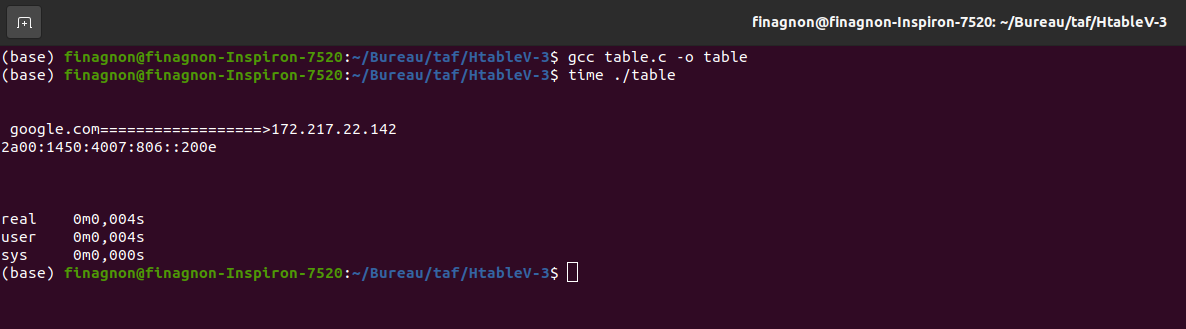
\includegraphics[scale = 0.5]{figures/sequent.png}
\captionof{Figure 5}{ : Figure montrant l'exécusion séquentielle de notre programme.}
\\
Dans cette dernière série de figure nous verrons le temps en réponse de la version parallèle:\\\\
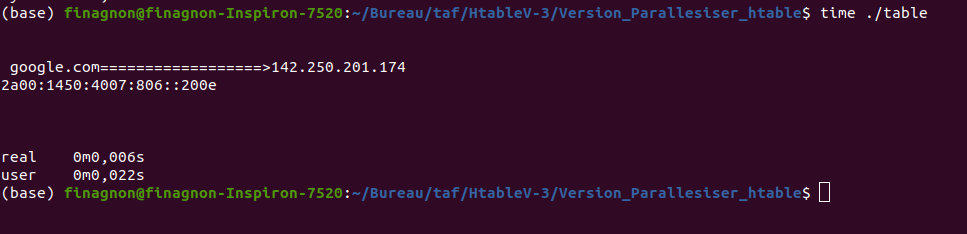
\includegraphics[scale = 0.5]{figures/paral.png}
\captionof{Figure 6 }{ : Temps de réponse en parallèle}
\newpage
\section{Organisation et déroulement}

Notre travaille était scindé périodiquement sur le dépôt suivant un fichier pdf vient étayer l'organisation du travail.
https://github.com/sirdelta/ppn-dns

\subsection{Structure du projet}

\quad Pour rendre le plus cohérent possible notre solution, nous avons tenu a organiser notre dossier source de sorte à ce que chaque fichier soit spécifique à une activité bien précise dans le déroulement de notre programme. Ainsi, le dossier \textit{src} du projet contient les répertoires suivants :
\begin{itemize}
    \item Le répertoire \textit{data}, contenant les éléments relatifs à l’envoie et à la réception de paquets de données DNS, ainsi que le stockage de ces données échangées. Il s’agit essentiellement de la définition des structures de données et routines qui permettent de les manipuler.
    \item Le répertoire \textit{net}, contenant les éléments permettant les échanges de données entre client et serveur DNS. On y trouve les principales fonctions qui orchestre l’envoi, la réception et le traitement des requêtes aboutissant à la résolution noms.
    \item La répertoire \textit{config}, contenant essentiellement des entêtes dans lesquelles sont définis des variables de tailles et de limites essentielles au bon fonctionnement du programme.
\end{itemize}

\quad Les principaux fichiers sources du projet sont rangés à la racine du dossier \textit{src}. Le dossier *tests* contient uniquement les fichiers sources des tests de validation sur les méthodes et routines situées dans le dossiers \textit{src}. Les exécutables générés sont rangés dans le répertoire \textit{build}.
\section{répartition des tâches}
\quad Afin de mener à bien notre projet, nous avons tenu à nous répartir les tâches en tenant compte des compétences de chacun en programmation réseau et en gestion de projet. Les tâches ont été attribuée de la manière suivante :
\begin{itemize}
    \item Y. Kapko : Réalisation de la table de hachage pour le stockage des données échangées ; mise en place d’un système de cache ; test de validation ; étude de performance ; Proposition du rapport.
    \item S. Koné : Création des structures de données relatives aux requêtes DNS, implémentations d’un client et d’un serveur DNS
    \item H. MLahara : Réalisation d’un système de \textit{log} pour le suivi du déroulement du programme.
\end{itemize}

\newpage
\section{Niveau d’achèvement}

\quad À l’issue de notre travail, nous sommes parvenu à réaliser un un client et un serveur DNS qui communique et s’échanger des données, une table de hachage qui stocke les informations échanger et une première approche pour le système de log. Cependant, notre programme rencontre quelques limites.

\subsection{Limites du projet}

\quad En effet, le communication client/serveur n’est pas réalisée dans le strict respect de la RFC 1035 décrivant les spécification du protocole DNS. Il n’ y a pas de limite de taille imposée pour les transferts de données d’un nœud du réseau à un autre. De plus, les paquets sont échangés par l’intermédiaire du protocole TCP, et non du protocole UDP, comme préciser dans la RFC. Nous n'avons donc pas pour l'instant proposé un remplacement direct de DNS mais une première itération d'un proxy DNS sur protocole ad-hoc. Cependant, cela permet déjà de vérifier notre capacité à fournir la fonctionnalité clef-valeur, un point que nous allons étendre de manière distribuée dans le futur.

\subsection{Travaux Futurs}

\quad Pour le prochain semestre, nous envisageons les points suivants :
\begin{itemize}
    \item L'amélioration du système de cache par la mise en place d'un système plus simple
    \item Lancement d'application réelle MPI sur notre proxy (implémentation de la PMI1);
    \item L'ajout de tests de validations supplémentaires sur les méthodes et routines ;
    \item Parallélisation de la table de hachage,  
    \itdem La sérialisation de données échanger entre le client et le serveur DNS ;
    \item Une analyse de performance de notre solution.
    % \item L'utilisation de mode "w + b" pour l'ouverture d'un fichier binaire en lecture/écriture;
    % \item La relecture d’un caractère avec la fonction "ungetc" et le Positionnement dans un fichier.
\end{itemize}

\newpage
\section*{Conclusion}
\addcontentsline{toc}{section}{Conclusion}

\quad Pour conclure, nous pouvons dire dans un premier temps que le protocole DNS est un mécanisme efficace qui permet la résolution de noms et d’adresses IP dans un réseau distribué. Nous nous sommes penchés sur PMIx et DNS afin de chercher les points communs, notre exploration a menée à la réalisation d'un proxy DNS permettant de mimer les fonctionnalités de ces deux composants en même temps. Notre but étant de nous inspirer du meilleur de chacun de ces composants. Notre approche initiale présentée dans ce document a montré la faisabilité de ce point, cependant comme mentionné dans la section précédentes certaines limitations persistent et nous souhaitons les adresser durant le prochain semestre.

\quad Du point de vue des compétences, la réalisation de ce projet nous a permis d’acquérir des connaissances en programmation réseau. En effet, nous avons appris à mettre en pratiques des notions complexes en étudiant des documents techniques et en faisant des recherches sur des domaines très poussés du calcul haute performance.

\newpage
\section*{Références}
\addcontentsline{toc}{section}{Références}
\bibitem{wikipedia},https://fr.wikipedia.org/wiki/Domain_Name_System\\
	  \emph{: Article sur le DNS}.\\
	   16 avril 2020 à 08:26.
  
%\begin{thebibliography}{}
\bibitem{wikipedia},https://datatracker.ietf.org/doc/html/rfc1035\\
	  \emph{: RFC1035 MEMO sur le DNS}.
	  \emph{
	   Network Working Group                                     P. Mockapetris
Request for Comments: 1035                                           ISI
         
                                                         November 1987
                                                         }
                                                         
                                                         https://benhoyt.com/writings/hash-table-in-c/

https://www.python.org/dev/peps/pep-0456/

https://www.youtube.com/watch?v=2Ti5yvumFTU

https://www.youtube.com/watch?v=b3dv_BA5B4E&t=2450s

\newpage
\section*{Annexes}
\addcontentsline{toc}{section}{Annexes}
Nous avons sur ce dépôt les différents dépot de notre travail:\\
https://github.com/sirdelta/ppn-dns


\end{document}
